\documentclass[12pt]{article}
\usepackage{amsmath}
\usepackage{amssymb,amsfonts,amsthm}
\usepackage[english]{babel}
\usepackage[utf8]{inputenc}
\usepackage[T1]{fontenc}
\usepackage{hyperref}
\usepackage{xcolor}
\usepackage{graphicx} 
\usepackage{caption}
\usepackage{subcaption}
\usepackage{listings}
\usepackage{anysize}
%\usepackage{polski}

\graphicspath{ {img/} }
\title{Arduino – układy wejścia/wyjścia (SW lab01)}
\author{Olga Gerlich ..., Kamil Kałużny 148121 grupa I1.2}
\marginsize{2.5cm}{2.5cm}{0cm}{3cm}

\definecolor{codegreen}{rgb}{0,0.6,0}
\definecolor{codegray}{rgb}{0.5,0.5,0.5}
\definecolor{codepurple}{rgb}{0.58,0,0.82}
\definecolor{backcolour}{rgb}{0.95,0.95,0.92}

\lstdefinestyle{mystyle}{
	backgroundcolor=\color{backcolour},   
	commentstyle=\color{codegreen},
	keywordstyle=\color{magenta},
	numberstyle=\tiny\color{codegray},
	stringstyle=\color{codepurple},
	basicstyle=\ttfamily\footnotesize,
	breakatwhitespace=false,         
	breaklines=true,                 
	captionpos=b,                    
	keepspaces=true,                 
	numbers=left,                    
	numbersep=5pt,                  
	showspaces=false,                
	showstringspaces=false,
	showtabs=false,                  
	tabsize=2
}

\lstset{style=mystyle}

\begin{document}
	\maketitle
	\section{Dobór rezystancji dla diody zielonej, żółtej i czerwonej}
	\subsection{Zadanie ,,blink''}
	\begin{figure}[h!]
		\begin{center}
			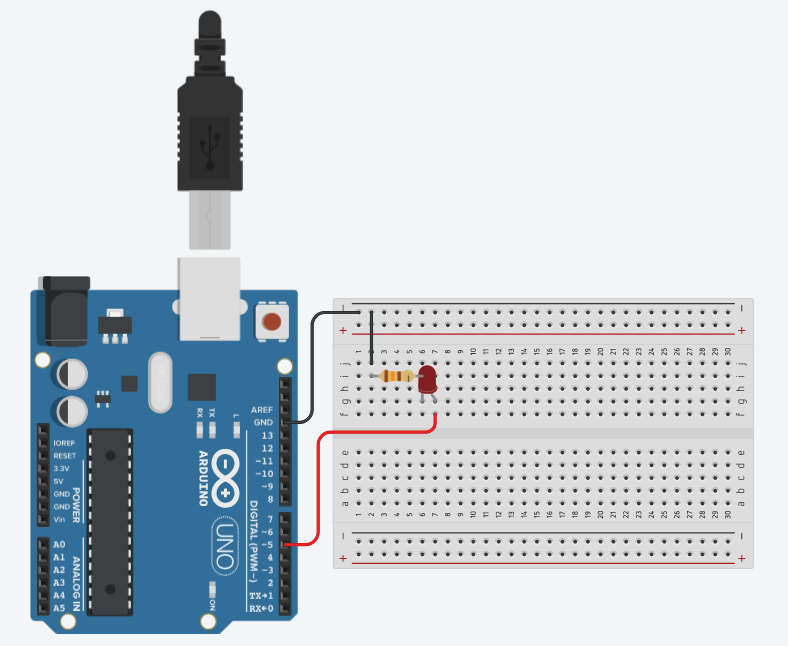
\includegraphics[scale=0.4]{01_blink.png}
			\caption*{Schemat podłączenia diody do Arduino}
		\end{center}
		\begin{lstlisting}[language=C++]
			void setup() {
				pinMode(5, OUTPUT);
			}
			
			void loop() {
				digitalWrite(5, HIGH);
				delay(1000);
				digitalWrite(5,LOW);
				delay(1000);
			}
		\end{lstlisting}
		\caption*{Kod źródłowy}
	\end{figure}
	\subsection{Obliczenia rezystancji dla diód o różnych kolorach}
	%TODO
	\section{Dioda + przycisk}
	\begin{figure}[h!]
		\begin{center}
			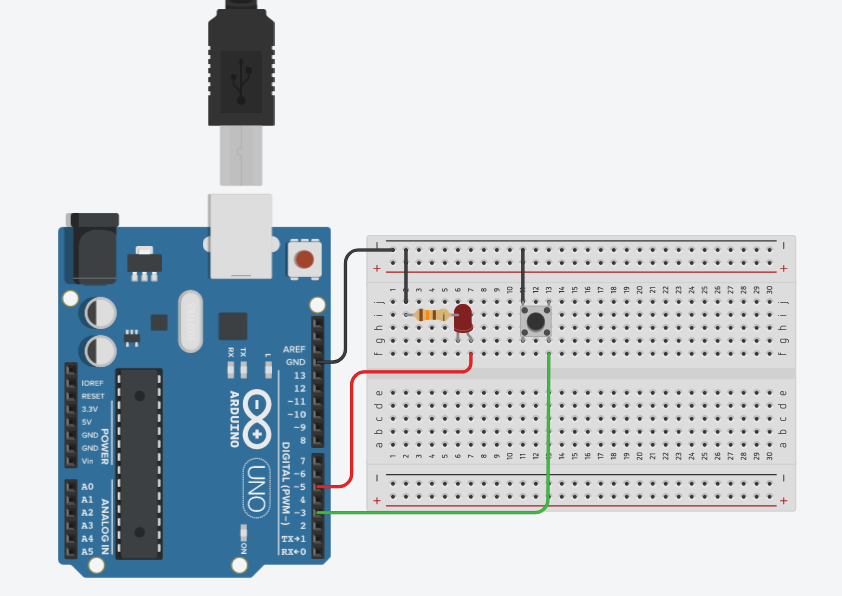
\includegraphics[scale=0.4]{02_button.png}
			\caption*{Schemat podłączenia diody oraz przycisku do Arduino}
		\end{center}
		\begin{lstlisting}[language=C++]
		int btn = HIGH;
		
		void setup() {
			pinMode(5, OUTPUT);
			pinMode(3, INPUT_PULLUP);
			digitalWrite(5, LOW);
		}
		
		void loop() {
			btn = digitalRead(3);
			if (btn == LOW){
				digitalWrite(5, HIGH);
			}
			else{
				digitalWrite(5,LOW);
			}
		}
		\end{lstlisting}
		\caption*{Kod źródłowy}
	\end{figure}
	
	\newpage
	\section{Potencjometr + dioda + Monitor Portu Szeregowego}
	\subsection{Zadanie ,,potencjometr i dioda''}
	\begin{figure}[h!]
		\begin{center}
			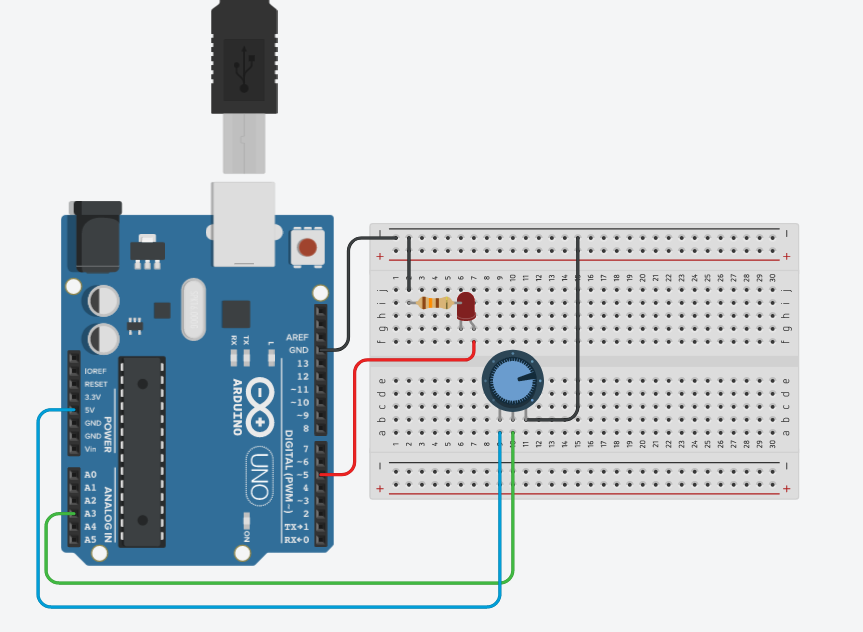
\includegraphics[scale=0.4]{03_serial_conn.png}
			\caption*{Schemat podłączenia diody oraz potencjometru do Arduino}
		\end{center}
		\begin{lstlisting}[language=C++]
			void setup() {
				pinMode(5, OUTPUT);
				pinMode(A3, INPUT);
				digitalWrite(5, LOW);
				Serial.begin(9600);
			}
			
			void loop() {
				Serial.println(analogRead(A3));
				if (analogRead(A3) >= 600){
					digitalWrite(5, HIGH);
				} else{
					digitalWrite(5,LOW);
				}
			}
		\end{lstlisting}
		\caption*{Kod źródłowy}
	\end{figure}
	% Zrzut ekranu z monitora portu szeregowego
	% TODO nie wiem czy to robimy w sumie czy wywalone
	\subsection{Opis działania przetwornika A/C}
	% TODO
	\newpage
	\begingroup
	\hypersetup{hidelinks}
	\tableofcontents
	\endgroup
\end{document}

